\documentclass[a4paper,12pt]{article}

\usepackage[backend=bibtex]{biblatex} 
\usepackage{geometry} 
\usepackage{titling} 
\usepackage{titlesec}
\usepackage[english]{babel} 
\usepackage[hidelinks]{hyperref} 
\usepackage{listings} 
\usepackage{xcolor}
\usepackage{graphicx} 
\usepackage{forest} 
\usepackage{tikz-qtree} \usepackage[siunitx, european, straightvoltages, cute inductors]{circuitikz} 
\usepackage{setspace} \usepackage{ragged2e}

\addbibresource{ref.bib}

\definecolor{codegreen}{rgb}{0,0.6,0} 
\definecolor{codegray}{rgb}{0.5,0.5,0.5}
\definecolor{codepurple}{rgb}{0.58,0,0.82} 
\definecolor{backcolour}{rgb}{0.95,0.95,0.92}

\lstdefinestyle{mystyle}{
	backgroundcolor=\color{backcolour}, 
	commentstyle=\color{codegreen}, 
	keywordstyle=\color{magenta},
	numberstyle=\tiny\color{codegray}, 
	stringstyle=\color{codepurple}, 
	basicstyle=\ttfamily\footnotesize,
	breakatwhitespace=false, breaklines=true, captionpos=b, keepspaces=true, numbers=left, numbersep=5pt,
	showspaces=false, showstringspaces=false, showtabs=false, tabsize=8
}
\lstset{style=mystyle}

\tikzstyle{startstop} = [rectangle, rounded corners, minimum width=3cm, minimum height=1cm,text centered, draw=black, fill=red!30]
\tikzstyle{io} = [trapezium, trapezium left angle=70, trapezium right angle=110, minimum width=0cm, minimum height=1cm, text centered, draw=black, fill=blue!30]
\tikzstyle{process} = [rectangle, minimum width=3cm, minimum height=1cm, text centered, draw=black, fill=orange!30]
\tikzstyle{subroutine} = [rectangle, minimum width=3cm, minimum height=1cm, text centered, draw=black, fill=yellow!30, double distance=1]
\tikzstyle{decision} = [diamond, minimum width=3cm, minimum height=1cm, text centered, draw=black, fill=green!30]
\tikzstyle{arrow} = [thick,->,>=stealth]


\titleformat{\section} {\Huge} {} {0em} {}[\titlerule] 
\geometry{a4paper,total={170mm,257mm},left=25mm,right=25mm,}

\author{Lucas Standen} 
\title{Creating a simple temprature sensing circuit}

\begin{document} 
\maketitle

\newpage
\tableofcontents 
\newpage

\setlength{\parskip}{1em}

{\setlength{\parindent}{0cm}
	\section{System Planning} 
	\subsection{Problem analysis} 
	My circuit will sense temperature, and will be taking into consideration pet owners, worried about their homes over-heating 
	for their pets, this will be especially helpful for owners of sensitive pets such as fish. People who own these pets often 
	leave them at home alone, which can be deadly on summer days, my device plans to alert the owner, and can be attached to other 
	systems such as a cooling system.

	My system, will flash an LED and pulse a buzzer to make it clear that it is too hot, have an indicator to tell
	the user that something has gone wrong, and have a pin to free to attach to an external system.  It will have a
	adjustment dial to change the threshold, so the user can specify what temperature is too hot.

	\subsection{Who is it for?} 
	My project will be used by pet owners, focussing on fish, to keep the tank at the
	correct temperature.  This is a broad range of people as many people own fish\cite{FISH}. Many fish die due to
	their tanks getting too hot, especially in the summer, my project is perfect for these fish owners.

	\section{Design specification} 
	\subsection{System Design} 
	The project will need to do the following things:
	\begin{description}
		\item[] Read the temprature
		\item[] Compare the temprature to a known value
		\item[] The output is a flashing led and buzzer
		\item[] The output is a flashing led and buzzer
	\end{description}

	My system will contain the following components to
	function: 
	\begin{description}
		\item[Mircocontroller] This will be used to control all the other components \item[Thermistor] This will
			sense the temperature 
		\item[Potentiomiter] This will set the activation threshold 
		\item[Red, Green and Amber LED's] These will indicate the state of the device 
		\item[Buzzer] This will indicate that it is too
			hot 
		\item[Button] This will reset the device
	\end{description} 
	With these components I will make a circuit that can be used to sense and warn a user about
	high temperatures. The design will revolve around the micro controller, with everything else coming off it as a
	sub system like so:

	\begin{center} 
		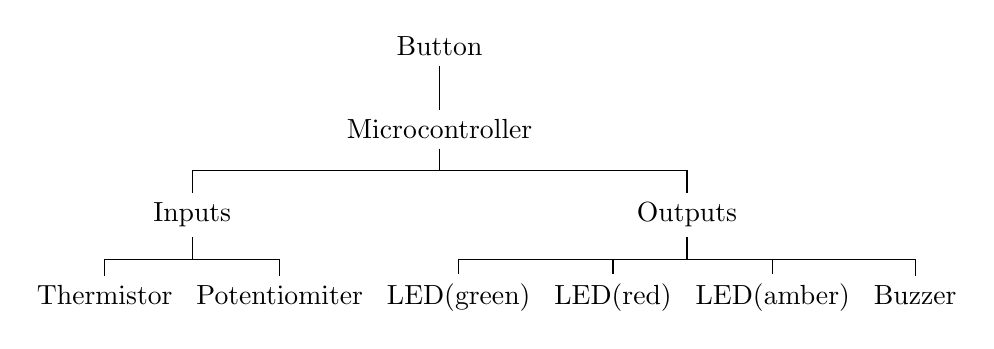
\begin{tikzpicture} 
			\tikzset{edge from parent/.style={draw,edge from parent path={(\tikzparentnode.south)-- +(0,-8pt)-| (\tikzchildnode)}}} 
			\Tree
			[.Button
			[.Microcontroller
			[.Inputs
			[.Thermistor ] [.Potentiomiter ]
			] [.Outputs
			[.LED(green) ] [.LED(red) ] [.LED(amber) ] [.Buzzer ]
			]
			]
			]
		\end{tikzpicture} 
	\end{center}

	As one can see a button will control the Microcontroller, by drawing all the current that the power supply
	can through the button, one can make the Microcontroller reset. The Microcontroller will have 2 inputs, and
	4 outputs. The potentiomiter will be used to set the threshold in which the warnings begin, this will be done
	inside the microcontroller, with a subtraction between the Thermistor value, and the potentiometer value. The
	needed outputs will pulse to be especially clear that something is wrong.

	\subsection{Flowchart}
	Here is my code, build into an abstracted flow chart, to make the reading of the program easier. 
	It is spread across 2 pages, to ensure it is big enough to read.

	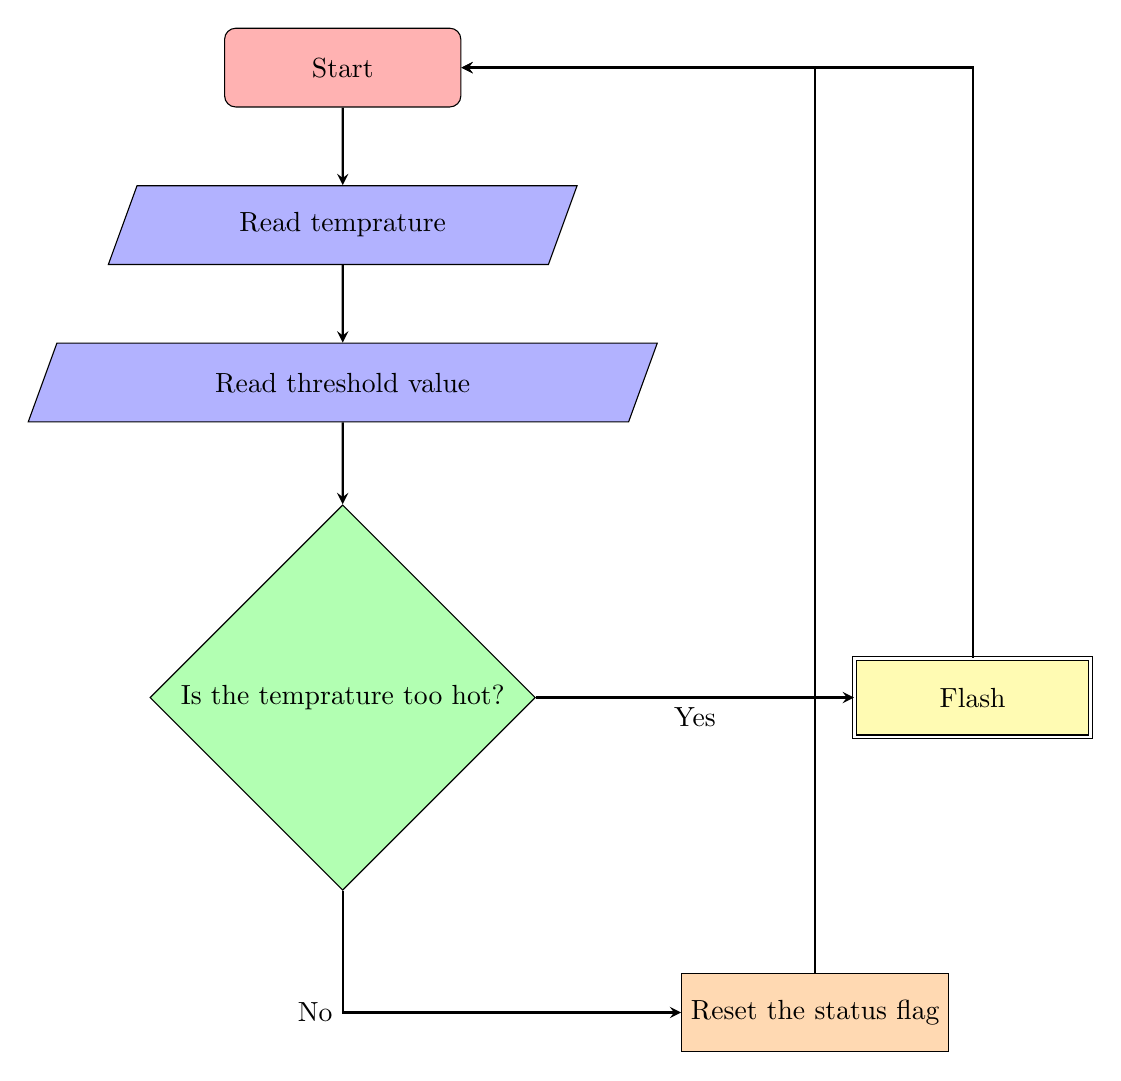
\begin{tikzpicture}[node distance=2cm]
		\node (start) [startstop] {Start};
		\node (in1) [io, below of=start] {Read temprature};
		\node (in2) [io, below of=in1] {Read threshold value};
		\node (dec1) [decision, below of=in2, yshift=-2cm] {Is the temprature too hot?};
		\node (sub1) [subroutine, right of=dec1, xshift=6cm] {Flash};
		\node (proc1) [process, below of=dec1, yshift=-2cm, xshift=6cm] {Reset the status flag};


		\draw [arrow] (start) -- (in1);
		\draw [arrow] (in1) -- (in2);
		\draw [arrow] (in2) -- (dec1);
		\draw [arrow] (dec1) -- node[anchor=north] {Yes} (sub1);
		\draw [arrow] (sub1) |- (start);
		\draw [arrow] (dec1) |- node[anchor=east] {No} (proc1); 
		\draw [arrow] (proc1) |- (start);
	\end{tikzpicture}
	\newpage
	\begin{tikzpicture}[node distance=2cm]
		\node (flash) [subroutine, below of=dec1, yshift=-4cm] {Flash};
		\node (proc2) [process, below of=flash] {Set counter to 5};
		\node (out1) [io, below of=proc2] {Set LED and buzzer on};
		\node (proc3) [process, below of=out1] {Wait 1 second};
		\node (proc4) [process, below of=proc3] {Decrement 1 from the counter};
		\node (dec2) [decision, below of=proc4, yshift=-1cm] {Is counter == 0};
		\node (out3) [io, below of=dec2, yshift=-1cm] {Set LED and buzzer off};
		\node (return) [subroutine, below of=out3] {Return};
		\node (out2) [io, right of=dec2, xshift=6cm] {Set LED and buzzer off};
		\node (proc5) [process, above of=out2] {Wait 1 second};

		\draw [arrow] (flash) -- (proc2);
		\draw [arrow] (proc2) -- (out1);
		\draw [arrow] (out1) -- (proc3);
		\draw [arrow] (proc3) -- (proc4);
		\draw [arrow] (proc4) -- (dec2);
		\draw [arrow] (dec2) -- node[anchor=north] {No} (out2);
		\draw [arrow] (dec2) -- node[anchor=east] {Yes} (out3);
		\draw [arrow] (out3) -- (return);
		\draw [arrow] (out2) -- (proc5);
		\draw [arrow] (proc5) |- (out1);
	\end{tikzpicture}



	\subsection{How will it function?} 
	Bellow is the diagram for my circuit, it works mostly via the code on the
	micro controller, so this is just connecting things between live and the microcontroller.   
	\begin{flushleft}
		\begin{circuitikz}
			\draw (-8,5) to[short,o-o] (8,5){}; % power rail 
			\draw (0,5) node[vcc]{5V};

			\draw (-8,-6) to[short,o-o] (8,-6){}; % ground rail 
			\draw (0,-6) node[ground]{};

			\draw (0,3) to[short,o-] (7,3){}; % push button 
			\draw (7,3) to[push button,-o] (7,-6){};

			\ctikzset{multipoles/thickness=4} 
			\ctikzset{multipoles/external pins thickness=2} 
			\draw (0,0)node[dipchip,
				num pins=18, external pins width=0.3, 
				external pad fraction=3, 
				scale=1.8, 
				rotate=90](Micro){
				\rotatebox{-90}{PICAXE 18m2}}; % micro controller

			\draw (-7, 5) to[thermistor,a=\tiny{100K},o-o] (-7,0){}; % thermistor 
			\draw (-7, 0) to[resistor,a=\tiny{100K},o-o] (-7,-6){}; % thermistor divider resistor

			\draw (-7, 0) to[short, o-] (-6,0){}; %thermistor divider wire 
			\draw (-6, 0) to[short, -] (-6,3){}; 
			\draw(-6, 3) to[short, -] (-4, 3){}; 
			\draw (-4, 3) to[short, -] (Micro.pin 18){};

			\draw (-8, 5) to[potentiometer, a=\tiny{10K}, -] (-8, -2){}; 
			\draw (-8, -2) to[short, -] (-8, -6){};

			\draw (-7.5, 1.5) to[short, o-] (-5, 1.5){}; % potentiometer wire 
			\draw (-5, 1.5) to[short,-] (-5, 4){};
			\draw (-5, 4) to[short,-] (-3, 4){}; 
			\draw (-3, 4) to[short, -] (Micro.pin 17){};


			\draw (Micro.pin 14) to[short,-o] (0,5){}; %microcontroller live 
			\draw (Micro.pin 5) to[short,-o](0,-6){}; %microcontroller ground

			\draw (Micro.pin 6) to[empty led] (1, -4){}; %output red 
			\draw (Micro.pin 7) to[buzzer] (2, -6){}; %output buzzer 
			\draw (Micro.pin 8) to[empty led] (3, -4){}; %output amber 
			\draw (Micro.pin 9) to[empty led] (4, -4){}; %output green

			\draw (1,-4) to[resistor,-o,a=\tiny{220}] (1,-6){}; % output resistor 
			\draw (3,-4) to[resistor,-o,a=\tiny{220}] (3,-6){}; % output resistor 
			\draw (4,-4) to[resistor,-o,a=\tiny{220}] (4,-6){}; % output resistor
		\end{circuitikz} 
	\end{flushleft} 
	The way this works is the potential divider on the
	left feeds into the micro controller which performs a comparison between it and the potentiometer, using the ADC
	pins on the pic chip. The button seen on the right is being used as a reset switch, for a short time, it can
	cut short circuit the system, cutting power to the microcontroller, effectively acting as a reset switch. The
	outputs at the bottom are in order; a red LED that flashes when the circuit detects it is too hot; a buzzer that
	flashes at the same time; an amber LED that turns on after the flashing has stopped to inform the user that it
	was too hot at some point; and a green status LED to inform the user that all is working.  

	\subsection{The code}
	Bellow is the code for the micro controller. It is 59 lines long and commented. It contains 12 unique instructions.
	\lstinputlisting[]{./final.asm} 
	This code starts with an initialisation section, that sets the micro controller's input and output pins to do
	the correct things. Then it defines a subroutine that flashes the LED and buzzer and sets the status led. And
	finally the main function runs in a loop to continue checking if it is too hot. 
	\section{System Realisation} 
	\subsection{Circuit realisation}
	PUT CIRCUIT PHOTO HERE

	Here is my finished design prototyped on a bread board, I have cut the wires to an adequate length to ensure it is cleanly made.
	I left the potential divider open, as I changed what value components I was using many times.

	\subsection{Calibrating the sensors} 
	\subsection{Results}

	\section{System Evaluation} 
	\subsection{Did it work?} 
	\subsection{What could go better?}

	\newpage

	\printbibliography 
} 
\end{document}
